\documentclass[a4paper,11pt]{article}

\usepackage[T1]{fontenc}
\usepackage[utf8]{inputenc}
\usepackage{graphicx}
\usepackage{xcolor}

\renewcommand\familydefault{\sfdefault}
\usepackage{tgheros}
%\usepackage[defaultmono]{droidmono}

\usepackage{amsmath,amssymb,amsthm,textcomp}
\usepackage{enumerate}
\usepackage{multicol}
\usepackage{tikz}

\usepackage{verbatimbox}
\usepackage{enumitem} 

\usepackage{geometry}
\geometry{left=25mm,right=25mm,%
bindingoffset=0mm, top=20mm,bottom=20mm}


\linespread{1.3}

\newcommand{\linia}{\rule{\linewidth}{0.5pt}}

% custom theorems if needed
\newtheoremstyle{mytheor}
    {1ex}{1ex}{\normalfont}{0pt}{\scshape}{.}{1ex}
    {{\thmname{#1 }}{\thmnumber{#2}}{\thmnote{ (#3)}}}

\theoremstyle{mytheor}
\newtheorem{defi}{Definition}

% my own titles
\usepackage[compact]{titlesec}
\makeatletter
\renewcommand{\maketitle}{
\begin{center}
\vspace{1ex}
{\huge \textsc{\@title}}
\vspace{1ex}
\\
\linia\\
\@author \hfill \@date
\vspace{2ex}
\end{center}
}
\makeatother
%%%

% custom footers and headers
\usepackage{fancyhdr}
\pagestyle{fancy}
\lhead{}
\chead{}
\rhead{}
\lfoot{Project Assignment \textnumero{} 2}
\cfoot{}
\rfoot{Page \thepage}
\renewcommand{\headrulewidth}{0pt}
\renewcommand{\footrulewidth}{0pt}
%

% code listing settings
\usepackage{listings}
\usepackage{enumitem}
\setitemize{itemsep=0pt}
\lstset{
    language=Python,
    basicstyle=\ttfamily\small,
    aboveskip={1.0\baselineskip},
    belowskip={1.0\baselineskip},
    columns=fixed,
    extendedchars=true,
    breaklines=true,
    tabsize=4,
    prebreak=\raisebox{0ex}[0ex][0ex]{\ensuremath{\hookleftarrow}},
    frame=lines,
    showtabs=false,
    showspaces=false,
    showstringspaces=false,
    keywordstyle=\color[rgb]{0.627,0.126,0.941},
    commentstyle=\color[rgb]{0.133,0.545,0.133},
    stringstyle=\color[rgb]{01,0,0},
    numbers=left,
    numberstyle=\small,
    stepnumber=1,
    numbersep=10pt,
    captionpos=t,
    escapeinside={\%*}{*)}
}
\renewcommand{\texttt}[1]{%
  \begingroup
  \ttfamily
  \begingroup\lccode`~=`/\lowercase{\endgroup\def~}{/\discretionary{}{}{}}%
  \begingroup\lccode`~=`[\lowercase{\endgroup\def~}{[\discretionary{}{}{}}%
  \begingroup\lccode`~=`.\lowercase{\endgroup\def~}{.\discretionary{}{}{}}%
  \catcode`/=\active\catcode`[=\active\catcode`.=\active
  \scantokens{#1\noexpand}%
  \endgroup
}

\setlength\parindent{0pt}
\setlength{\parsep}{0pt}
\setcounter{secnumdepth}{0}

\usetikzlibrary{calc,positioning,arrows}

%%%----------%%%----------%%%----------%%%----------%%%

\begin{document}

\author{Štěpánka Gennertová 451432, Marek Šanta 433772, Michal Pavúk 487550}
\date{\textit{2020-04-23}}
\title{Security Technologies\\\medskip
\large Project assignment \textnumero{} 2}

\maketitle
In this report we present our implementation of secure channel communication
protocol between the client application and the applet. It is based on a
standardised J-PAKE. In addition to the standard Diffie-Hellman key exchange,
whose functionality is contained within the protocol, J-PAKE provides mutual
authentication of both parties.

The Password Authenticated Key Exchange by Juggling (\emph{J-PAKE}) is a
password-authenticated key agreement protocol, that allows two parties to
establish private and authenticated communication, based on their shared
low-entropy password (in our case PIN).

Theoretical description of J-PAKE protocol defines a completely symmetrical
two-round key exchange. Such an exchange is impractical in scenarios where the
communication is initiated by one of the parties. Fortunately the authors of
the protocol recognize this issue and provide a three-pass variant of the
protocol. However due to technical limitations of the JavaCard platform, namely
missing support for extended APDUs in many environments (including JCardSim) we
split the data that would be transferred in a single response into 2 responses.
This has no effect on the overall security of the protocol.

\section{Protocol}
\label{sec:orgf0cf5bc}

For the purposes of this description we refer to the two communicating parties
as an application (running on host computer) and an applet (running on the
card).

The application initiates the communication with the card by selecting the
installed applet for secure data transmission. It then sends the \texttt{INIT} command
(INS: 01) with the required data.

\(E(F_p)\) is an elliptic curve over a finite field \(F_p\) where \(p\) is a
sufficiently large prime of order \(n\). Our implementation uses the prime256v1
curve. We use \(s\) to denote the shared secret (PIN).

\subsection{Phase 1}
\label{sec:org2d28cdf}

The application generates ephemeral private keys \(x_1\) and \(x_2\) from
\(\langle 1, n-1 \rangle\). It then selects the applet and sends the \texttt{INIT}
APDU.

The data contained within the \texttt{INIT} command are:
\begin{itemize}
\item \(G_1 = G^{x_1} \mod p\) and \(G_2 = G^{x_2} \mod p\)
\item \(V_{x_1}\), \(V_{x_2}\), \(r_{x_1}\) and \(r_{x_2}\) are components for
zero-knowledge proofs for \(x_1\) and \(x_2\) respectively
\end{itemize}

\subsection{Phase 2}
\label{sec:org6988486}

The applet verifies the ZKPs for \(x_1\) and \(x_2\). If the proofs are \textbf{NOT} valid
the applet responds with error code and the session initiation is terminated.
Otherwise it will, similarly to the application, randomly select an ephemeral
private keys \(x_3\) and \(x_4\) from \(\langle 1, n-1 \rangle\). It then responds with:
\begin{itemize}
\item \(G_3 = G^{x_3} \mod p\), \(G_4 = G^{x_4} \mod p\)
\item \(V_{x_3}\), \(V_{x_4}\), \(r_{x_3}\) and \(r_{x_4}\) as ZKPs for \(x_3\) and \(x_4\)
\end{itemize}

\subsection{Phase 3}
\label{sec:org3002721}

The application verifies ZKPs for \(x_3\) and \(x_4\) in case they
are \textbf{NOT} valid, the application terminates the session by deselecting the
applet (and clearing card's RAM in the process). Otherwise the application will
send the \texttt{FINISH} command, containing:
\begin{itemize}
\item \(A = (G_1 \cdot G_2 \cdot G_4)^{x_2 \cdot s} \mod p\)
\item A ZKP for \(x_2 \cdot s\)
\end{itemize}

\subsection{Phase 4}
\label{sec:org5bf3ea3}

Upon receiving the second APDU command, the applet verifies the proof for
\(x_2 \cdot s\). If the proof is valid, it responds with its generator \(B\):
\begin{itemize}
\item \(B = (G_1 \cdot G_2 \cdot G_3)^{x_4 \cdot s} \mod p\)
\item \(V_{x_4 \cdot s}\) and \(r_{x_4 \cdot s}\) as a ZKP for \(x_4 \cdot s\)
\end{itemize}

Now both parties will compute the common key material as follows:
\begin{itemize}
\item Application: \(K_a = (B - (g_4 \cdot [x_2 \cdot s])) \cdot x_2\)
\item Applet: \(K_b = (A - (g_2 \cdot [x_4 \cdot s])) \cdot x_4\)
\end{itemize}

At this point, the following equality holds true: \(K_a = K_b = G \cdot
    [(x_1+x_3)\cdot (x_2 \cdot x_4 \cdot s)]\) and both parties will use key
derivation function to derive a common session key \(k\). All subsequent
communication is then encrypted using the derived session key \(k\).

\section{Diagram}
\label{sec:org3052e42}

\begin{figure}[!htb]
 \centering
 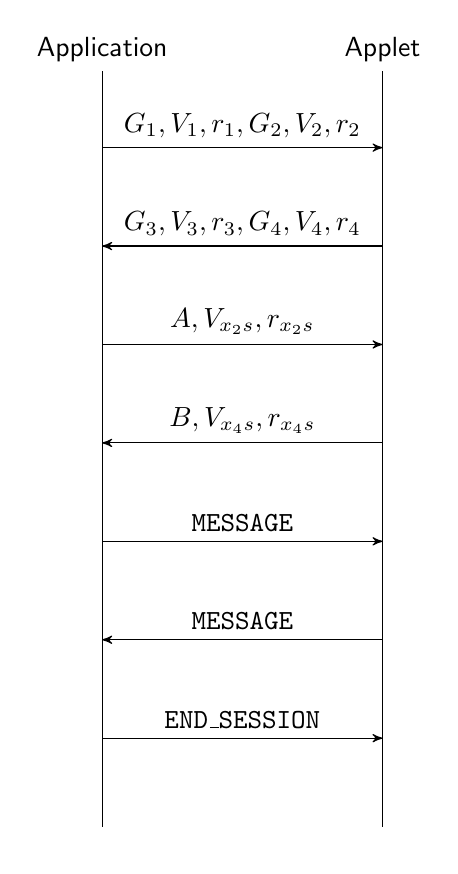
\begin{tikzpicture}[node distance=2cm,auto,>=stealth']
      \node[] (A) {Applet};
      \node[left = of A] (B) {Application};
      \node[below of=A, node distance=10cm] (A_ground) {};
      \node[below of=B, node distance=10cm] (B_ground) {};

      \draw (A) -- (A_ground);
      \draw (B) -- (B_ground);
      \draw[->] ($(B)!0.125!(B_ground)$) -- node[above,scale=1,midway]{\(G_1, V_1, r_1, G_2, V_2, r_2\)} ($(A)!0.125!(A_ground)$);
      \draw[<-] ($(B)!0.25!(B_ground)$) -- node[above,scale=1,midway]{\(G_3, V_3, r_3, G_4, V_4, r_4\)} ($(A)!0.25!(A_ground)$);
      \draw[->] ($(B)!0.375!(B_ground)$) -- node[above,scale=1,midway]{\(A, V_{x_2s}, r_{x_2s}\)} ($(A)!0.375!(A_ground)$);
      \draw[<-] ($(B)!0.5!(B_ground)$) -- node[above,scale=1,midway]{\(B, V_{x_4s}, r_{x_4s}\)} ($(A)!0.5!(A_ground)$);
      \draw[->] ($(B)!0.625!(B_ground)$) -- node[above,scale=1,midway]{\texttt{MESSAGE}} ($(A)!0.625!(A_ground)$);
      \draw[<-] ($(B)!0.75!(B_ground)$) -- node[above,scale=1,midway]{\texttt{MESSAGE}} ($(A)!0.75!(A_ground)$);
      \draw[->] ($(B)!0.875!(B_ground)$) -- node[above,scale=1,midway]{\texttt{END\_SESSION}} ($(A)!0.875!(A_ground)$);
      %\draw[<-] ($(B)!1!(B_ground)$) -- node[above,scale=1,midway]{\texttt{END\_SESSION}} ($(A)!1!(A_ground)$);
 \end{tikzpicture}
\end{figure}

\section{Commands, responses and messages}
\label{sec:org37877ff}

\begin{center}%[!htb]
%\centering
\resizebox{\textwidth}{!}{\begin{tabular}{llrrrlll}
Message & CLA / Code & INS & P1 & P2 & L\textsubscript{c} & Data field & L\textsubscript{e}\\
\hline
SELECT & 00 & 04 & 04 & 00 &  & AID & \\
INIT J-Pake 1 & b0 & 01 & 00 & 00 & C4 & \(G_1, V_1, r_1, G_2, V_2, r_2\) & C4\\
I-RESPONSE J-Pake 2 & 90 00 & - & - & - & - & \(G_3, V_3, r_3, G_4, V_4, r_4\) & \\
FINISH J-Pake 3 & b0 & 02 & 00 & 00 & 63 & \(A, Vx2s, rx2s\) & 63\\
F-RESPONSE J-Pake 4 & 90 00 & - & - & - & - & \(B, V_{x_4s}, r_{x_4s}\) & \\
END\_SESSION & b0 & 03 & 00 & 00 & - & - & -\\
MESSAGE & b0 & 04 & 00 & 00 & variable & encrypted message data & \\
\end{tabular}}
\end{center}

The \texttt{MESSAGE} APDUs contain data encrypted with the derived session key \(k\) and have a following format:
\begin{center}
\begin{tabular}{rrll}
Offset & Size & Value & Description\\
\hline
0 & 1 & counter 00-FF & \\
1 & 2 & checksum & ALG\_ISO3309\_CRC16\\
3 & 1 & length 00-FD & remaining length of the data\\
4 & length 00-FD & any & message contents\\
4+length & 256-4-length & padding & random bytes\\
\end{tabular}
\end{center}

\section{Implementation}
\label{sec:org9ff6715}

The purpose of the counter is to detect and prevent dropping, and replaying of
the encrypted messages. The counter is valid for the duration of the session and
starts at the value of 0. It increments with each successfully received command
(as indicated by the response code). Should either party receive a message with
the counter value lower than its internal session counter, the session is
immediately terminated. On the other hand, should the counter be larger than the
internal one, some packets were dropped by the adversary and the session is
terminated.

While the attacker has knowledge of the counter value, they cannot modify the
value of the counter due to the presence of encryption. The semantics regarding
the checksum mismatch are set by the application utilizing the channel.

The \texttt{END\_SESSION} message does not require any kind of verification. While we
are aware that this simplification allows the attacker to finish a session
prematurely, we decide to leave it as-is, since the attacker can simply cut the
connection entirely.


\end{document}